%%% 20131217 iwata adopt to report form
\def\thisdir{science/hizpeak/}

%\documentclass[]{article}
%\usepackage{graphicx}
%\usepackage{amsmath,amssymb}
%\usepackage{natbib,aas_macros}
%\citestyle{aa}
%\bibliographystyle{apj}


%\oddsidemargin   -0.2cm
%\evensidemargin  -0.2cm
%\topmargin       -0.2cm
%\textwidth        16.5cm
%\textheight       22.0cm
%\parindent        11pt

\newcommand\lya{Ly$\alpha$}
\newcommand\ha{H$\alpha$}
\newcommand\hb{H$\beta$}
\newcommand\paa{Pa$\alpha$}
\newcommand\oii{[O~{\sc ii}]}
\newcommand\oiii{[O~{\sc iii}]}
\newcommand\nii{[N~{\sc ii}]}

\def\gsim{\mathrel{\raise0.35ex\hbox{$\scriptstyle >$}\kern-0.6em % Greater/squiggles
\lower0.40ex\hbox{{$\scriptstyle \sim$}}}}
\def\lsim{\mathrel{\raise0.35ex\hbox{$\scriptstyle <$}\kern-0.6em % Less than/squiggles 
\lower0.40ex\hbox{{$\scriptstyle \sim$}}}}
\def\msun{{\rm M}$_{\odot}$}

%\begin{document}
%\noindent
%\Large
\section{Galaxy Formation at Its Peak Epoch Revealed by ULTIMATE-Subaru
 Project \label{sec:highzpeak}}

\noindent
%\\vspace{5mm}
%\large
\begin{center}
%% Authors
{\bf Tadayuki Kodama (NAOJ), Yusei Koyama (NAOJ), Ken-ichi Tadaki (NAOJ),
and Michael Balogh (Univ. of Waterloo, Canada)}
\end{center}
\vspace{0.5cm}

\normalsize
%%      Introduction (summary of past researches, key questions)
\subsection{Introduction}
\subsubsection{The peak epoch of galaxy formation}

Recent observations have established that star-formation (SF) and AGN
activities come to peaks at $1\lsim z\lsim 3$ (cosmic look-back time of 8--11 Gyrs)
\citep[e.g.,][]{madau96,lilly96,hopkins06}.
This means that the bulk of stellar contents within
present-day galaxies were formed in that peak epoch of cosmic SF
history. It is therefore crucial to study these rapidly growing
galaxies at this peak epoch, in order to fully
understand the key physical drivers of galaxy formation and evolution.

One of the important discoveries in the recent extra-galactic
astronomy is the tight relationship between galaxy stellar mass and
star-formation rate (SFR), which is often referred to as the ``star
formation main sequence'' \citep[e.g.,][]{Brinchmann04, elbaz07, daddi07}.
The SF main sequence is now investigated out
to $z\gsim 2$ \citep[e.g.,][]{whitaker12}, and it is shown that the
SFR of $z\sim 2$ galaxies (for a given stellar mass) is $\sim$30 times
higher than those in the present-day universe. It is reported that the
scatter around the SF main sequence is relatively small at all redshifts
($\sim$0.2--0.3~dex), which implies that galaxy stellar mass is an
important parameter regulating SF activity of galaxies.

However, the scatter around the main sequence reflects the variation
of gas accretion history of galaxies, hence it is important to
identify the origin of the scatter and understand the key parameter
that makes the strongest impact on the gas accretion history of
galaxies. \citet{wuyts11} studied how the galaxy structure and the
mode of SF activity depend on the position on the SFR--mass diagram.
They find that the upper envelope of SF main sequence is dominated by
dusty (i.e.\ high SFR$_{\rm IR}$/SFR$_{\rm UV}$ ratio) galaxies (Fig. 2)
with high sersic index ({\it n}) (Fig.\ 1), suggesting a rapid build-up
of mass in the nuclear regions of these systems, due for example to
galaxy-galaxy interactions/mergers \citep{wuyts11}.
This kind of studies---linking {\it global} and {\it internal} properties
of galaxies---will become more and more important for understanding 
``how galaxies grow'' in the early universe (see also Section~*1.2*).

Another important parameter that drives galaxy evolution is
``environment''. It is well established that galaxy properties are
strongly dependent on environment, known as the morphology--density,
color--density, or SFR--density relations in the local universe 
\citep[e.g.,][]{dressler1980, lewis2002, gomez2003}.
Recent 
observational studies have shown that the environment strongly affects
the ``fraction'' of red/quenched galaxies, while the environmental
effect seems to be milder for SF activities {\it amongst} SF galaxies
\citep{balogh2004,peng2010}. A more recent study by \citet{koyama13b}
extend this idea up to $z\sim 2$ by comparing
H$\alpha$-selected galaxies in clusters and field environments
\citep[Fig.3,][]{koyama13b}.
These studies suggest that the environmental effect instantly shut down SF
activity of galaxies once the truncation process is started
so that they do not appear as ``being-truncated'' galaxies and do not change
the location of the main sequence of {\it star-forming} galaxies.

\subsubsection{Internal structures of forming galaxies}

The high-resolution imaging by $Hubble\ Space\ Telescope$ (HST) allows
us to study evolution of galaxy morphologies in distant universe.
For galaxies at $z>1.5$, near-infrared (NIR) observations are essential 
to sample the rest-frame optical lights, tracing the distribution of stellar mass. 
NIR high-resolution imagings have shown that massive quiescent galaxies 
at $z\sim2$ tend to be extremely compact compared to local ones with 
the same stellar mass \citep[e.g.,][]{vandokkum08}, suggesting 
the inside-out scenario; dense core are first formed by dissipational processes 
such as gas rich mergers and outer parts are subsequently built up by 
dry minor mergers \citep[e.g.,][]{vandokkum10}. 
However, \citet{vandokkum13} 
investigate the evolution of surface density profiles for Milky-Way-like
galaxies from $z=2.5$ to $z=0$ and find that bulges form in lockstep
with disks to $z\sim1$. This result rules out the inside-out 
growth for less massive Milky-Way-like galaxies and needs some sort of
physical mechanisms such as bar instabilities or clump migration to
explain the simultaneous formation of bulges and disks.

Star-forming galaxies at the peak epoch of galaxy formation actually tend 
to have irregular, clumpy morphologies unlike the present-day galaxies 
on the Hubble sequence \citep{elmegreen05}. Although such 
clumpy structures are often seen in both rest-frame UV and optical
wavelengths \citep{guo12}, the kinematics of ionized gas show ordinary
disks with symmetric rotation of $v_\mathrm{rot}\sim200-300$ km s$^{-1}$ 
\citep{genzel06}. Many of them also exhibit large local velocity
dispersions of $\sigma=30-90$ km s$^{-1}$, suggesting that the gas disks
commonly have random motions.

In the past several years, the efficient gas supply through cold streams along 
filamentary structures is suggested to be a preferred mechanism to account for 
enhancement in SFRs, clumpy structures embedded in ordinary rotational disks, 
and large velocity dispersions \citep{dekel09}.
The steady, narrow, cold gas streams penetrate the shock-heated media of 
massive dark matter haloes and continuously supply a large amount of gas 
to the inner regions of star-forming galaxies. The smooth streams maintain 
dense gas-rich disks, as observed in CO observations \citep{tacconi10}.
In such a gas rich disk, a small gas perturbation in the radial direction would 
grow up and fragment into giant clumps by a gravitational instability.
Then, the internal gravitational interactions within a perturbed disk generate
turbulences and the velocity dispersion becomes progressively larger. 
Though any direct observational evidence for cold gas streams has not been 
found yet, this may account for all the differences in the properties between 
high-$z$ and local galaxies.

The clumpy structures of galaxies suggest a new scenario of bulge formation. 
In the numerical simulations, clumps formed from gravitational instabilities can 
migrate toward a galaxy center as a result of their mutual interactions and of 
dynamical friction against the host disk, and coalesce into a young bulge 
\citep[e.g.,][]{inoue12}.
This is an unusually efficient process to carry a large amount of gas and 
star from galactic disks to bulge components. Then, a starburst would be 
induced at the center by a collision between the clumps in a manner similar 
to a major merger \citep{barnes96}. However, we have very little 
knowledge about it observationally.

\subsubsection{Mahalo-Subaru Survey Project}

In order to explore this critical epoch for galaxy formation,
near-infrared (NIR) observations are essential,
as the rest-frame optical light, where most of the information
on stellar populations exist, is all redshifted into NIR regime. 
However large systematic observations at NIR which achieve both depth
and width have been limited due to high background noise (including the
forest of OH sky lines) in the ground-based NIR observations and limited
field of view of NIR instruments on large telescopes. 
The situation is dramatically improving recently because of the advent
of various wide-field imagers and spectrographs on 8--10m telescopes. 
MOIRCS and FMOS on Subaru are the first examples, and MOSFIRE on Keck,
HAWK-I/KMOS on VLT, and FLAMINGOS-2 on Gemini are bursting out
recently. 

By utilizing the large field of view of MOIRCS (4$'$$\times$7$'$), 
we firstly conducted deep and wide NIR imaging of 4 promising
proto-clusters at 2$\lsim$$z$$\lsim$3 \citep{kodama07}.
Based on the $J-K_s$ vs $K_s$ colour-magnitude diagrams, we revealed
that the red sequence of cluster galaxies at the massive-end above
10$^{11}$\msun are just emerging between $z=3$ and 2, indicating that we
are entering the epoch of massive galaxies formation in proto-clusters.  
We have also been conducting the ``Mahalo-Subaru'' project 
\citep[MApping HAlpha and Lines of Oxygen with Subaru;][]{kodama13}, 
in which we targeted proto-clusters at 1.45$<$$z$$<$2.53 
\citep{hayashi10, hayashi11, hayashi12, tadaki12, koyama13a},
%(Hayashi et al. 2010; 2011; 2012; Tadaki et al. 2012;
%Koyama et al. 2013a), 
and an un-biased general field SXDF-CANDELS 
\citep[$z$=2.19 and 2.53 slices;][]{tadaki13, tadaki14}.
We made a series of narrow-band (NB) filters for this specific purpose,
and we have been mapping out star-forming emission line galaxies (\ha)
down to dust-free SFR of 10~\msun/yr in narrow redshift slices
associated to the clusters or in the general field. 
The great advantage of using narrow-band technique is that we can make a
nearly star formation rate limited sample with high completeness, and
the selection bias is minimized. 

Based on this unique sample, we have been investigating the properties
of star forming galaxies at their peak epoch of formation. 
In particular, our survey area in SXDF is fully covered by the HST
CANDELS survey \citep{grogin11} 
and the high resolution optical and NIR images are both freely available 
(0.18$''$ resolution in H-band corresponds to 1.5kpc in physical scale
at $z\sim2$). 
We have identified $\sim$100 \ha\ emitters in total at $z$=2.19 and 2.53
using NB2095 and NB2315, respectively.
By measuring star formation rates (SFR) accurately based on \ha\ line
fluxes and dust extinction estimated from SED, 
we find that the star formation activity is significantly higher for a
given stellar mass (M$_{*}$) than the local SFR--M$_{*}$ relation of
star forming galaxies (called as the main sequence) by a factor of 30
\citep{koyama13b}.
Moreover, the HST images have revealed that about 40\% of massive star
forming galaxies ($>$2$\times$10$^{10}$M$_{\odot}$) have clumpy
structures \citep[Fig.\ 4;][]{tadaki13, tadaki14}, 
despite of the fact that many of these galaxies show ordered disk-like
rotation. They are either external mergers or internal clumpy galaxies
fragmented by gravitational instability of gas rich disks 
\citep{genzel11} fed by cold streams \citep{dekel09}.
Since the clumps are likely to migrate towards galaxy center due to
dynamical friction, they are probably intimately linked to bulge
formation in disk galaxies. In any case, this indicates that galaxy
formation at its peak epoch is not simple but involves some complicated
physical processes, and such irregularity is probably responsible, at
least partly, for very high star formation and AGN activities seen at
this epoch. 

\subsubsection{Current limitations}

The ultimate goals of the studies of galaxy formation and evolution are
to unveil (1) the physical driver of the overall decline of SF
activity over the last $\sim$10~Gyrs (mainly for field galaxies), 
(2) the physics of SF quenching of galaxies (mainly for group/cluster
galaxies) and (3) the physical process of bulge formation. 
For this purpose, we require a large, statistical sample of
galaxies selected from a variety of environments in the distant Universe.
The data currently available are too small
because of limited FoV and sensitivity of the existing observational facilities.
%In particular, NB-based emission-line survey is extremely
%powerful to construct an uniformly selected, high-$z$ SF galaxy samples.
%Our pilot survey with Subaru (MAHALO-Subaru; Kodama et al.
%2013; Tadaki et al. 2011) used H$\alpha$ and/or [OII] emitters in
%(proto-)clusters and general fields to study environmental dependence
%of SF galaxy properties at $z>1$. From this survey, we have found a
%strong evidence that SF galaxies in proto-cluster environments (at
%$z\gsim 2$) tend to be more massive and have higher SFR (Hayashi et
%al. 2012; Koyama et al. 2013a). Such red/massive SF galaxies in
%distant cluster environments represent an accelerated galaxy evolution
%(or enhanced mode of SF activity) in dense environment. The basic but
%exciting approach is to quantify the frequency of star-bursting
%galaxies as well as quiescent galaxies at various redshifts and
%environments.
Moreover, the ground-based seeing limited surveys
cannot resolve internal physics of galaxy formation and evolution.
The great combination of wide FoV and
sharp imaging quality to be achieved with ULTIMATE-Subaru will
thus revolutionize the situation.

%%      New windows to be opened with Subaru GLAO
\subsection{New windows to be opened with Subaru GLAO}

Mean spatial resolusion of 0.2$''$ at K-band to be achieved with GLAO
corresponds to 1.6kpc in physical scale for galaxies at the peak epoch
($1<z<3$). We aim to spatially resolve internal structures of extended
galaxies, in particular we will begin to resolve and separate internal
clumps (with a typical size of $\sim$1kpc) 
which are frequently recognized in star-forming galaxies at this epoch.
Such high-resolution analyses have recently been conducted intensively
with HST imaging (WFPC2, ACS) and AO-assisted IFU spectroscopy 
(e.g., SINFONI/VLT, OSIRIS/Keck, NIFS/Gemini).
However, HST imaging is limited to broad-bands and upto H$_{160}$-band,
a bit too short for us to trace stellar-mass distribution in $z>2$
galaxies. Also, AO-assisted multi-object spectroscopy (MOS) is not yet
available at all. Given these current limitations, high resolution
studies of distant galaxies should be expanded as follows: 
(1) Wavelength coverage should be extended to 2.5$\mu$m (K-band) so that 
we can trace stellar mass distribution of galaxies even at $z>2$ up to
$z\sim4$. 
(2) Narrow-band imaging should be conducted to trace star forming
galaxies with H$\alpha$ emitters ($z<2.6$) and [OIII] emitters
($z<3.7$). NB imaging is in fact very powerful for NIR observations with
ground-based telescopes as we can achieve a high sensitivity by
targeting clean wavelength ranges in between the OH sky lines.
(3) AO-assisted MOS observations should be made possible in order to make
a statistical sample of resolved spectroscopy of high-$z$ galaxies.

%%      Proposed observations (obs mode, targets, required # of nights)
\subsection{Proposed observations}

\subsubsection{Overview}

We propose an unprecidentedly large (e.g., 2 deg$^2$), high reslution, imaging 
(broad-band and narrow-band) and spectroscopic surveys of the peak epoch of galaxy 
formation with the ULTIMATE-Subaru (*Section~3.1 and 3.2*). We remind that the 
ULTIMATE-Subaru offers a uniformly good 0.2 arcsec resolution in $K$-band across 
$\sim$15 arcmin field in each pointing. The proposed 2~deg$^2$ field size corresponds
to a comoving volume of 7$\times$10$^5$ Mpc$^3$ per $\Delta$$z$=1. 
Although we expect the survey will contain a few progenitors of massive galaxy 
clusters of M$_{\rm cluster}$$>$10$^{14}$\msun, 
%Therefore, it allows us to average over the cosmic variance and at the same time to 
%explore environmental dependence of galaxy properties. 
we also propose a more systematic ``targeted'' survey of distant
(proto-)clusters to complement our survey in general fields
(*Section~3.3*).  

\subsubsection{The ULTIMATE-Subaru legacy survey: imaging}

The primary goal of the legacy survey with ULTIMATE-Subaru is to construct the
largest, unbiased sample of distant galaxies with an excellent imaging quality
ever established. Assuming a field of view of the new instrument of 200
arcmin$^2$,  36 pointings will be needed to tile the entire 2 deg$^2$
field. We will use at least 3 narrow-band filters (corresponding to
$z\sim1.5$, 2.0, and 2.5 for \ha, and $z\sim2.0$, 2.6, 3.3 for \oiii)
and K$_s$-band in each pointing, and integrate for 3 hours on each NB
filter to reach down to \ha-based SFR=15\msun/yr  
at $z=2$ (dust extinction corrected) and 0.5 hrs at K$_s$-band.
From our past experience with Mahalo-Subaru, we will be able to detect
$\sim$100 \ha, and $\sim$20 \oiii, emitters at $z=2$ and $z=3$ respectively
in each pointing, and thus more than 10,000 \ha\ emitters and 2,000
\oiii\ emitters in total at $1.5<z<2.5$ and $2<z<3.3$ respectively over
the 2 sq.\ deg. In this way, the total requested time will be $\sim$50
nights for this imaging part of the survey.

The current resolved rest-frame UV images by HST/ACS cannot really tell
us the internal star forming activities because of large dust
extinction. The AO-assisted H$\alpha$ narrow-band imaging is ideal for
mapping  star-forming regions within individual galaxies. We can
directly confirm  where dusty star formation is occurring because the
H$\alpha$  emission line is less affected by dust extinction. 
To demonstrate what can be studied from high-resolution H$\alpha$
imagings,  we show images of some star-forming galaxies at $z=2.5$ in
Figure 4 \citep{tadaki14}.
They consists of a central clump with red color in $I_{814}-H_{160}$
and some off-center blue clumps as clearly seen in the HST images.
While the rest-frame UV light is concentrated to the blue clumps, 
the H$\alpha$ flux traced by the narrow-band image is dominated 
by the central red clump. This is the clear evidence for the presence 
of dusty star-formation in the central red clump.  With AO-assisted 
narrow-band images, we will be able to trace the true distribution of 
star-forming activities within many of star-forming galaxies. This is a 
vital step to understanding the physical processes occurring in
star-forming galaxies at high-$z$. Moreover, the equivalent width of
H$\alpha$ line in each clump is the excellent tracer of its stellar
population age or specific star formation rate (sSFR).
By combining the H$\alpha$ equivalent width with ``dustiness'' in each  
clump, we can break the age-dustiness degeneracy of the clump properties  
as well as quantify the mode of star formation in each clump, and make a  
critical test for the clump migration and bulge formation scenario.

\subsubsection{The ULTIMATE-Subaru legacy survey: spectroscopy}

We also plan to do multi-slit spectroscopic follow-up observations with
some slit scans (e.g., 0.4$''$ slit $\times$ 3 scans) to spatially
resolve extended galaxies. Typical exposure time will be 5 hrs per scan,
and thus 36 pointings will take $\sim$50 nights to complete the
spctroscopic part. The high resolution spectroscopy will resolve
internal kinematics and physical states (ionized states, metallicities,
AGN contribution) of star-forming galaxies from the line ratios.

\subsubsection{Targeted cluster survey}

In addition to the general field survey described above, we also propose 
to carry out the identical observations towards distant ``cluster'' fields. 
The proposed wide-field unbiased 2~deg$^2$ survey described above will 
contain a few massive clusters, but it is clearly insufficient to fully 
assess environmental trends of galaxy properties as a function of e.g. 
cluster mass or richness. 
As we demonstrated in the MAHALO-Subaru project, the targeted cluster 
survey is the most efficient way to construct galaxy samples residing
in the high-density environments in the distant universe. 
We therefore propose to develop 
$\sim$10 NB filters with FWHM=120-220\AA (or more preferentially a
tunable filter system) designed to detect H$\alpha$ lines from
individual cluster fields. With the excellent  imaging quality over the
15$'$ FoV, the ULTIMATE-Subaru will allow us to spatially resolve
H$\alpha$ lines of {\it all} cluster members in the observed fields. The
number of known (proto-)clusters is currently very limited, but we
stress that the number of high-$z$ clusters will be significantly
increased by 2020s with a help of the on-going unprecedentedly  
large survey programmes with Hyper-Suprime-Cam. We target $\sim$20
proto-clusters at $1.5\lsim z\lsim 2.5$, and aim to obtain internal
H$\alpha$ maps of $\sim$2000 H$\alpha$ emitters in total. By comparing
the size of SF regions (through H$\alpha$ intensity map) and the stellar
mass density (drawn by K-band imaging) between cluster and field
galaxies, we will fully unveil the environmental impacts on the intenral
physics of high-$z$ galaxies. 

%%      Requirements for GLAO and instruments
\subsection{Requirements for GLAO and instruments}

The 0.2 arcsec seeing at K$_s$-band across a 15 arcmin field is required
for GLAO. A wide-field NIR instrument (camera and spectrograph) with a
field of view of 200 arcmin$^2$ is required for the proposed survey. 
Narrow-bands are essential, and at least 3 NB filters are mandatory to
investigate the redshift evolution over $1<z<3.5$.
Medium-band filters such as Y, J1, J2, H1, H2, H3, K1, K2, and K3 
with FWHM of 0.12--0.14$\mu$m are also useful to dramatically improve
the accuracy of photometric redshifts to $\Delta$$z/(1+z)$$<$0.02. 
As a spectrograph, 50--100 MOS slits in each FoV is optimal.

\begin{figure}%[htbp]
\centerline{
\includegraphics[width=120mm]{\thisdir figs/wuyts1.eps}
}
\caption{
Sersic index, $n$, is presented depending on the location on the
 SFR--M$_{*}$ diagram \citep{wuyts11}. 
The star forming galaxies which are deviated from the main sequence 
(solid white line) tend to have slightly higher $n$, indicating more
 light is present at the center due to a nucleated star burst. 
}
\label{fig:}
\end{figure}

\begin{figure}%[htbp]
\centerline{
\includegraphics[width=120mm]{\thisdir figs/wuyts2.eps}
}
\caption{
The ratio of SFR measured at infrared and that measured at UV, as an
 indicator of dust extinction is plotted depending on the location of
 the SFR--M$_{*}$ diagram \citep{wuyts11}. 
The star forming galaxies which are deviated from the main sequence 
(solid white line) tend to have higher SFR(IR)/SFR(UV) ratios,
 suggesting the presence of compact dusty star forming regions at the
 center. 
}
\label{fig:}
\end{figure}


\begin{figure}%[htbp]
\centerline{
\includegraphics[height=90mm]{\thisdir figs/koyama13.eps}
}
\caption{
Environmental dependence of the ``main sequence'' of star forming
 galaxies at $z\sim2$. 
Red filled circles and blue open squares show galaxies in a
 proto-cluster and those in the general field, respectively 
\citep{koyama13a}.
The location of the main sequence does not depend on
 environemnt. However, the galaxy distribution along the main sequence 
 does depend on the environment in the sense that star forming galaxies
 in the proto-cluster tend to be systematically more massive than 
those in the field.
}
\label{fig:}
\end{figure}

\begin{figure}%[htbp]
\centerline{
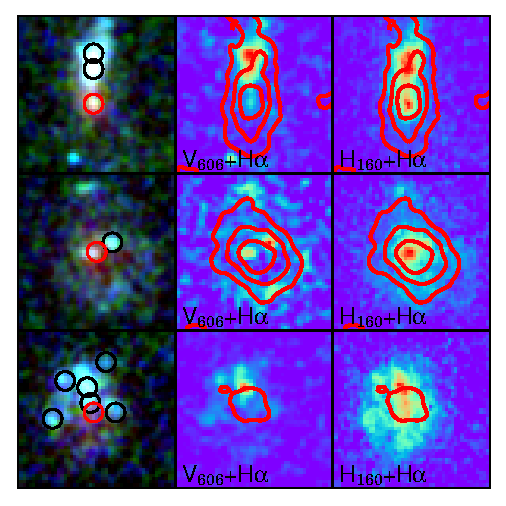
\includegraphics[height=80mm]{\thisdir figs/tadaki14.eps}
}
\caption{
Three H$\alpha$ emitters at $z$=2.16--2.53 with resolved dusty
 star-forming clumps. From left to right, three color images of
 V$_{606}$-I$_{814}$-H$_{160}$, V$_{606}$-band images, and
 H$_{160}$-band images are presented. Contours display the H$\alpha$
 flux density maps derived from NB (MOIRCS) and BB (WFCAM) images whose
 PSF sizes are matched to $\sim$0.7$''$. Red and black circles in right
 panels indicate the positions of the reddest clump nearest to the
 galactic center and other bluer clumps, respectively 
 \citep{tadaki14}.
}
\label{fig:}
\end{figure}


\bibliographystyle{apj}
\bibliography{\thisdir hizpeak}
%%\newpage
%%\bibliography{glao_report}

%\bibitem{madau96} Madau, P., et al., 1996, MNRAS, 283, 1388 
%\bibitem{lilly96} Lilly, S.~J., et al., 1996, ApJ, 460, L1 
%\bibitem{hopkins06} Hopkins, A.~M., \& Beacom, J.~F. 2006, ApJ, 651, 142 
%\bibitem{brinchmann04} Brinchmann, J., et al., 2004, MNRAS, 351, 1151 
%\bibitem{elbaz07} Elbaz, D., et al., 2007, A\&A, 468, 33 
%\bibitem{daddi07} Daddi, E., et al., 2007, ApJ, 670, 156 
%\bibitem{whitaker12} Whitaker K.~E., et al., 2012, ApJ, 754, L29 
%\bibitem{wuyts11} Wuyts S., et al., 2011, ApJ, 738, 106 
%\bibitem{dressler1980} Dressler A., 1980, ApJ, 236, 351 
%\bibitem{lewis2002} Lewis I., et al., 2002, MNRAS, 334, 673 
%\bibitem{gomez2003} G{\'o}mez P.~L., et al., 2003, ApJ, 584, 210 
%\bibitem{peng2010} Peng Y.-j., et al., 2010, ApJ, 721, 193 
%\bibitem{balogh2004} Balogh M., et al., 2004, MNRAS, 348, 1355 
%\bibitem{koyama13a} Kodama, Y., et al., 2013, MNRAS, 428, 1551
%\bibitem{koyama13b} Kodama, Y., et al., 2013, MNRAS, 434, 423

%\bibitem{kodama07} Kodama, T., et al., 2007, MNRAS, 377, 1717
%\bibitem{kodama13} Kodama, T., et al., 2013, IAUS295, in press
%\bibitem{genzel11} Genzel, R., et al., 2011, ApJ, 733, 101
%\bibitem{dekel09} Dekel, A., et al., 2009, Nature, 457, 451
%\bibitem{grogin11} Grogin, N., et al., 2011, ApJS, 197, 35
%\bibitem{tadaki13} Tadaki, K., et al., 2013, ApJ, in press
%\bibitem{tadaki14} Tadaki, K., et al., 2014, ApJ, in press

%\bibitem{vandokkum08} van Dokkum, P.~G., et al., 2008, ApJ, 677, L8
%\bibitem{vandokkum10} van Dokkum, P.~G., et al., 2010, ApJ, 709, 1018
%\bibitem{vandokkum13} van Dokkum, P.~G., et al., 2013, ApJ, 771, L35
%\bibitem{elmegreen05} Elmegreen \& Elmegreen 2005, ApJ, 627, 632
%\bibitem{guo12} Guo, Y., et al.,  2012, ApJ, 757, 120
%\bibitem{genzel06} Genzel, R., et al., 2006, Nature, 442, 786
%\bibitem{tacconi10} Tacconi, L.~J., et al., 2010, Nature, 463, 781
%\bibitem{inoue12} Inoue \& Saitoh 2012, MNRAS, 422, 1902
%\bibitem{barnes} Barnes \& Hernquist 1996, ApJ, 471, 115

%\end{document}
